\documentclass{article}

\usepackage{arxiv}
\usepackage[utf8]{inputenc}
\usepackage[T1]{fontenc}
\usepackage{hyperref}
\usepackage{url}
\usepackage{booktabs}
\usepackage{amsmath}
\usepackage{amsfonts}
\usepackage{array}
\usepackage{microtype}
\usepackage{graphicx}
\usepackage{xcolor}

\graphicspath{{figures/}}

\title{Can We Trust LLM Self-Explanations?\\
An Empirical Evaluation of Explanation-Support Faithfulness in Open-Source Large Language Models}

\author{
Yash Sakharam Gavade\\
Department of Computer Science\\
Universit\"at Trier\\
Trier, Germany\\
\texttt{s4yagava@uni-trier.de}
}

\begin{document}
\maketitle

\begin{abstract}
Large Language Models (LLMs) increasingly generate natural-language explanations together with their predictions, but fluent explanations are not necessarily reliable evidence of faithful reasoning. This paper presents a controlled empirical evaluation of self-generated explanations from three open-source instruction-tuned models: Qwen~2.5~3B, Llama~3.2~3B, and DeepSeek-R1 Distill Qwen~1.5B. Each model was evaluated on 100 fixed samples from GSM8K, CommonsenseQA, and StrategyQA using a standardized answer--explanation prompt, producing 900 responses in total. We measured answer accuracy, strict output-format success, generation time, and explanation length. We additionally constructed a balanced manual-analysis sample of 90 responses, containing equal numbers of correct and incorrect answers for every model--dataset pair, and scored explanation-support faithfulness, logical consistency, completeness, and primary failure type. DeepSeek-R1 Distill achieved the highest overall answer accuracy (52.33\%) and dominated GSM8K (80\%), while Qwen~2.5 achieved the best CommonsenseQA (76\%) and StrategyQA (60\%) accuracy. Llama achieved perfect strict-format success, whereas DeepSeek showed weaker instruction compliance (85.67\%). Across all models, explanations for correct answers received substantially higher faithfulness scores than explanations for incorrect answers. However, answer--explanation mismatches, unsupported justifications, hallucinations, arithmetic errors, and contradictory rationales remained common. The results show that explanation quality is strongly task-dependent and that natural-language self-explanations should be treated as behavioral justifications rather than direct evidence of a model's hidden internal reasoning.
\end{abstract}

\keywords{
Explainable Artificial Intelligence,
Large Language Models,
Faithfulness,
Self-Explanations,
Trustworthiness,
Open-Source LLMs,
Natural Language Processing
}


\section{Introduction}

Large Language Models (LLMs) can answer questions, solve mathematical problems, perform commonsense reasoning, and generate natural-language justifications for their outputs. Their explanations are often interpreted as evidence that the model has exposed the reasoning that led to a prediction. This interpretation is attractive because users receive not only an answer but also a human-readable basis for accepting, rejecting, or checking it. The rapid adoption of generative systems has therefore made explanation quality an increasingly important problem in Explainable Artificial Intelligence (XAI) \cite{gunning2019darpa,chang2024survey,schneider2024genxai}.

The apparent transparency of natural-language explanations is especially consequential in education, healthcare, finance, law, and scientific decision support. In these settings, users may rely on the explanation even when they cannot independently verify the output. A fluent explanation can increase trust despite containing unsupported claims, invalid arithmetic, or a conclusion that conflicts with the final answer. Human-centered XAI research has repeatedly emphasized that explanations should be evaluated not only for readability but also for their effect on user understanding and decision making \cite{miller2019explanation,brahman2022human,doshivelez2017rigorous}.

This motivates a distinction between \emph{plausibility} and \emph{faithfulness}. A plausible explanation is readable, coherent, and convincing to a human observer. A faithful explanation should accurately support the model's stated prediction and should not contradict the answer, invent facts, or omit critical steps. Strong causal faithfulness would require evidence that the explanation reflects the internal computation responsible for the prediction. Output inspection alone cannot establish that stronger claim \cite{turpin2023language,lanham2023measuring,parcalabescu2024measuring}. Consequently, this paper uses the narrower term \emph{explanation-support faithfulness}: the degree to which the visible explanation correctly, consistently, and sufficiently supports the visible final answer.

Recent work has shown that LLMs can produce fluent post-hoc rationales, biased chains of thought, and explanations that change without corresponding changes in the prediction \cite{madsen2024selfexplanations,paul2024making,matton2025walk,zaman2025causal}. These findings make it unsafe to equate textual reasoning with the model's hidden reasoning process. At the same time, visible explanations remain practically useful because they allow users and evaluators to detect contradictions, arithmetic mistakes, hallucinations, and incomplete reasoning. A behavioral evaluation therefore provides a useful intermediate step between simple answer accuracy and stronger causal analysis.

This study evaluates three open-source instruction-tuned models---Qwen~2.5~3B, Llama~3.2~3B, and DeepSeek-R1 Distill Qwen~1.5B---under a unified protocol. The models are compared on GSM8K, CommonsenseQA, and StrategyQA, representing mathematical, commonsense, and multi-step yes/no reasoning \cite{cobbe2021gsm8k,talmor2019commonsenseqa,geva2021strategyqa}. Every model receives the same fixed benchmark samples and the same structured answer--explanation prompt. The evaluation combines automatic answer scoring with a balanced manual analysis of explanation quality.

The study addresses four research questions:

\begin{enumerate}
    \item \textbf{RQ1:} How does answer accuracy vary across models and reasoning tasks?
    \item \textbf{RQ2:} How reliably do the models follow the required answer--explanation output format?
    \item \textbf{RQ3:} How does explanation-support faithfulness differ by model, dataset, and answer correctness?
    \item \textbf{RQ4:} Which explanation failure patterns occur most frequently?
\end{enumerate}

The following hypotheses guide the analysis:

\begin{itemize}
    \item \textbf{H1:} Models will show task-specific rather than uniform performance across datasets.
    \item \textbf{H2:} Explanations accompanying correct answers will receive higher faithfulness scores than explanations accompanying incorrect answers.
    \item \textbf{H3:} Reasoning-oriented models may achieve stronger mathematical accuracy but weaker format compliance and higher computational cost.
\end{itemize}

The main contributions are:

\begin{itemize}
    \item a controlled comparison of three open-source LLMs across three reasoning datasets and 900 total responses;
    \item a reproducible evaluation pipeline combining automatic answer scoring, strict format evaluation, and balanced manual explanation analysis;
    \item a lightweight rubric for explanation-support faithfulness, logical consistency, completeness, and primary failure type;
    \item an empirical analysis showing that answer accuracy, instruction compliance, runtime, and explanation quality vary substantially across models and tasks.
\end{itemize}

\section{Related Work}

\subsection{Explainable Artificial Intelligence}

XAI investigates methods that make machine-learning behavior understandable to humans. Classical post-hoc techniques such as LIME and SHAP estimate how input features contribute to a prediction \cite{ribeiro2016trust,lundberg2017unified}. These approaches have become standard reference points for local and global interpretability, but free-form language generation introduces additional challenges. An LLM can generate both a prediction and its explanation, meaning that the explanation is itself another model output rather than an independent analysis.

Interpretability research also warns against treating every human-readable artifact as a faithful account of a model's computation. Lipton describes interpretability as a broad and sometimes ambiguous concept, while Molnar provides a systematic account of model-agnostic interpretability methods and their assumptions \cite{lipton2018mythos,molnar2022interpretable}. Human-centered studies further show that explanation quality depends on the user's task and on whether the explanation enables appropriate reliance rather than merely increasing confidence \cite{miller2019explanation,brahman2022human}.

\subsection{Reasoning and Self-Explanation in LLMs}

Chain-of-Thought prompting encourages models to produce intermediate reasoning steps and can improve performance on arithmetic and symbolic tasks \cite{wei2022chain}. Subsequent work introduced self-consistency, least-to-most prompting, Tree of Thoughts, Graph of Thoughts, Program-of-Thoughts, and verifier-based approaches \cite{wang2023selfconsistency,zhou2023least,yao2023tree,besta2024graph,chen2023program,chen2023machine}. Other methods such as STaR, Reflexion, and Self-Refine use generated reasoning or feedback to improve later attempts \cite{zelikman2022star,shinn2023reflexion,madaan2023selfrefine}.

These methods demonstrate that explicit reasoning text can be useful for task performance, but usefulness does not imply faithfulness. The same model may generate a plausible rationale after committing to an answer, or it may produce reasoning that supports one conclusion while returning another. A self-explanation is therefore both a potential source of information and a potential source of misplaced trust.

\subsection{Evaluating Faithfulness of LLM Explanations}

Recent studies distinguish explanation plausibility from faithfulness. Stronger evaluation methods intervene on the prompt, rationale, or hidden computation and test whether model behavior changes in the expected direction \cite{turpin2023language,lanham2023measuring,zaman2025causal}. Other work evaluates whether self-explanations improve prediction, whether models ``walk the talk,'' or whether generated reasoning contains causal evidence rather than post-hoc justification \cite{madsen2024selfexplanations,paul2024making,matton2025walk}.

Automated hallucination and uncertainty methods provide complementary signals. SelfCheckGPT compares multiple generations to identify unsupported information, while semantic uncertainty methods aggregate meaning-level variation across outputs \cite{manakul2023selfcheckgpt,farquhar2024semantic}. These approaches are valuable at scale, but they do not fully capture logical contradictions, answer--explanation mismatches, or task-specific completeness. Manual evaluation remains useful for diagnosing such failures.

\subsection{Benchmarking and Open-Source Models}

Standardized evaluation frameworks such as HELM emphasize transparent reporting of prompts, datasets, and model settings \cite{liang2023helm}. Open-source model families make controlled reproduction more feasible. Qwen~2.5 provides instruction-tuned models across several sizes \cite{qwen2024qwen25}; Llama~3 offers a widely used family of open-weight models \cite{grattafiori2024llama3}; and DeepSeek-R1 introduces reasoning-oriented training and distilled variants \cite{deepseek2025r1}. Comparing these models under identical conditions helps separate model behavior from differences in prompt design or benchmark construction.

\subsection{Research Gap and Motivation}

Existing studies often focus on proprietary models, one dataset, one type of explanation, or one evaluation method. Direct comparison is difficult when prompts, decoding settings, sample selection, and scoring differ. This work addresses that gap through a fixed benchmark, deterministic decoding, a common parser, and the same evaluation rubric across three open-source models and three reasoning tasks. The goal is not to claim causal access to internal reasoning, but to measure whether visible explanations provide reliable behavioral support for visible answers.

\section{Methodology}

\subsection{Research Design}

The experiment follows the pipeline shown in Figure~\ref{fig:pipeline}. A fixed benchmark of 300 questions was constructed by sampling 100 examples from each dataset with random seed 42. The benchmark was frozen before final inference so that every model received the same questions in the same order. Each question produced a final answer and a concise explanation. Answers were scored automatically, while a balanced subset of explanations was manually annotated.

\begin{figure}[t]
    \centering
    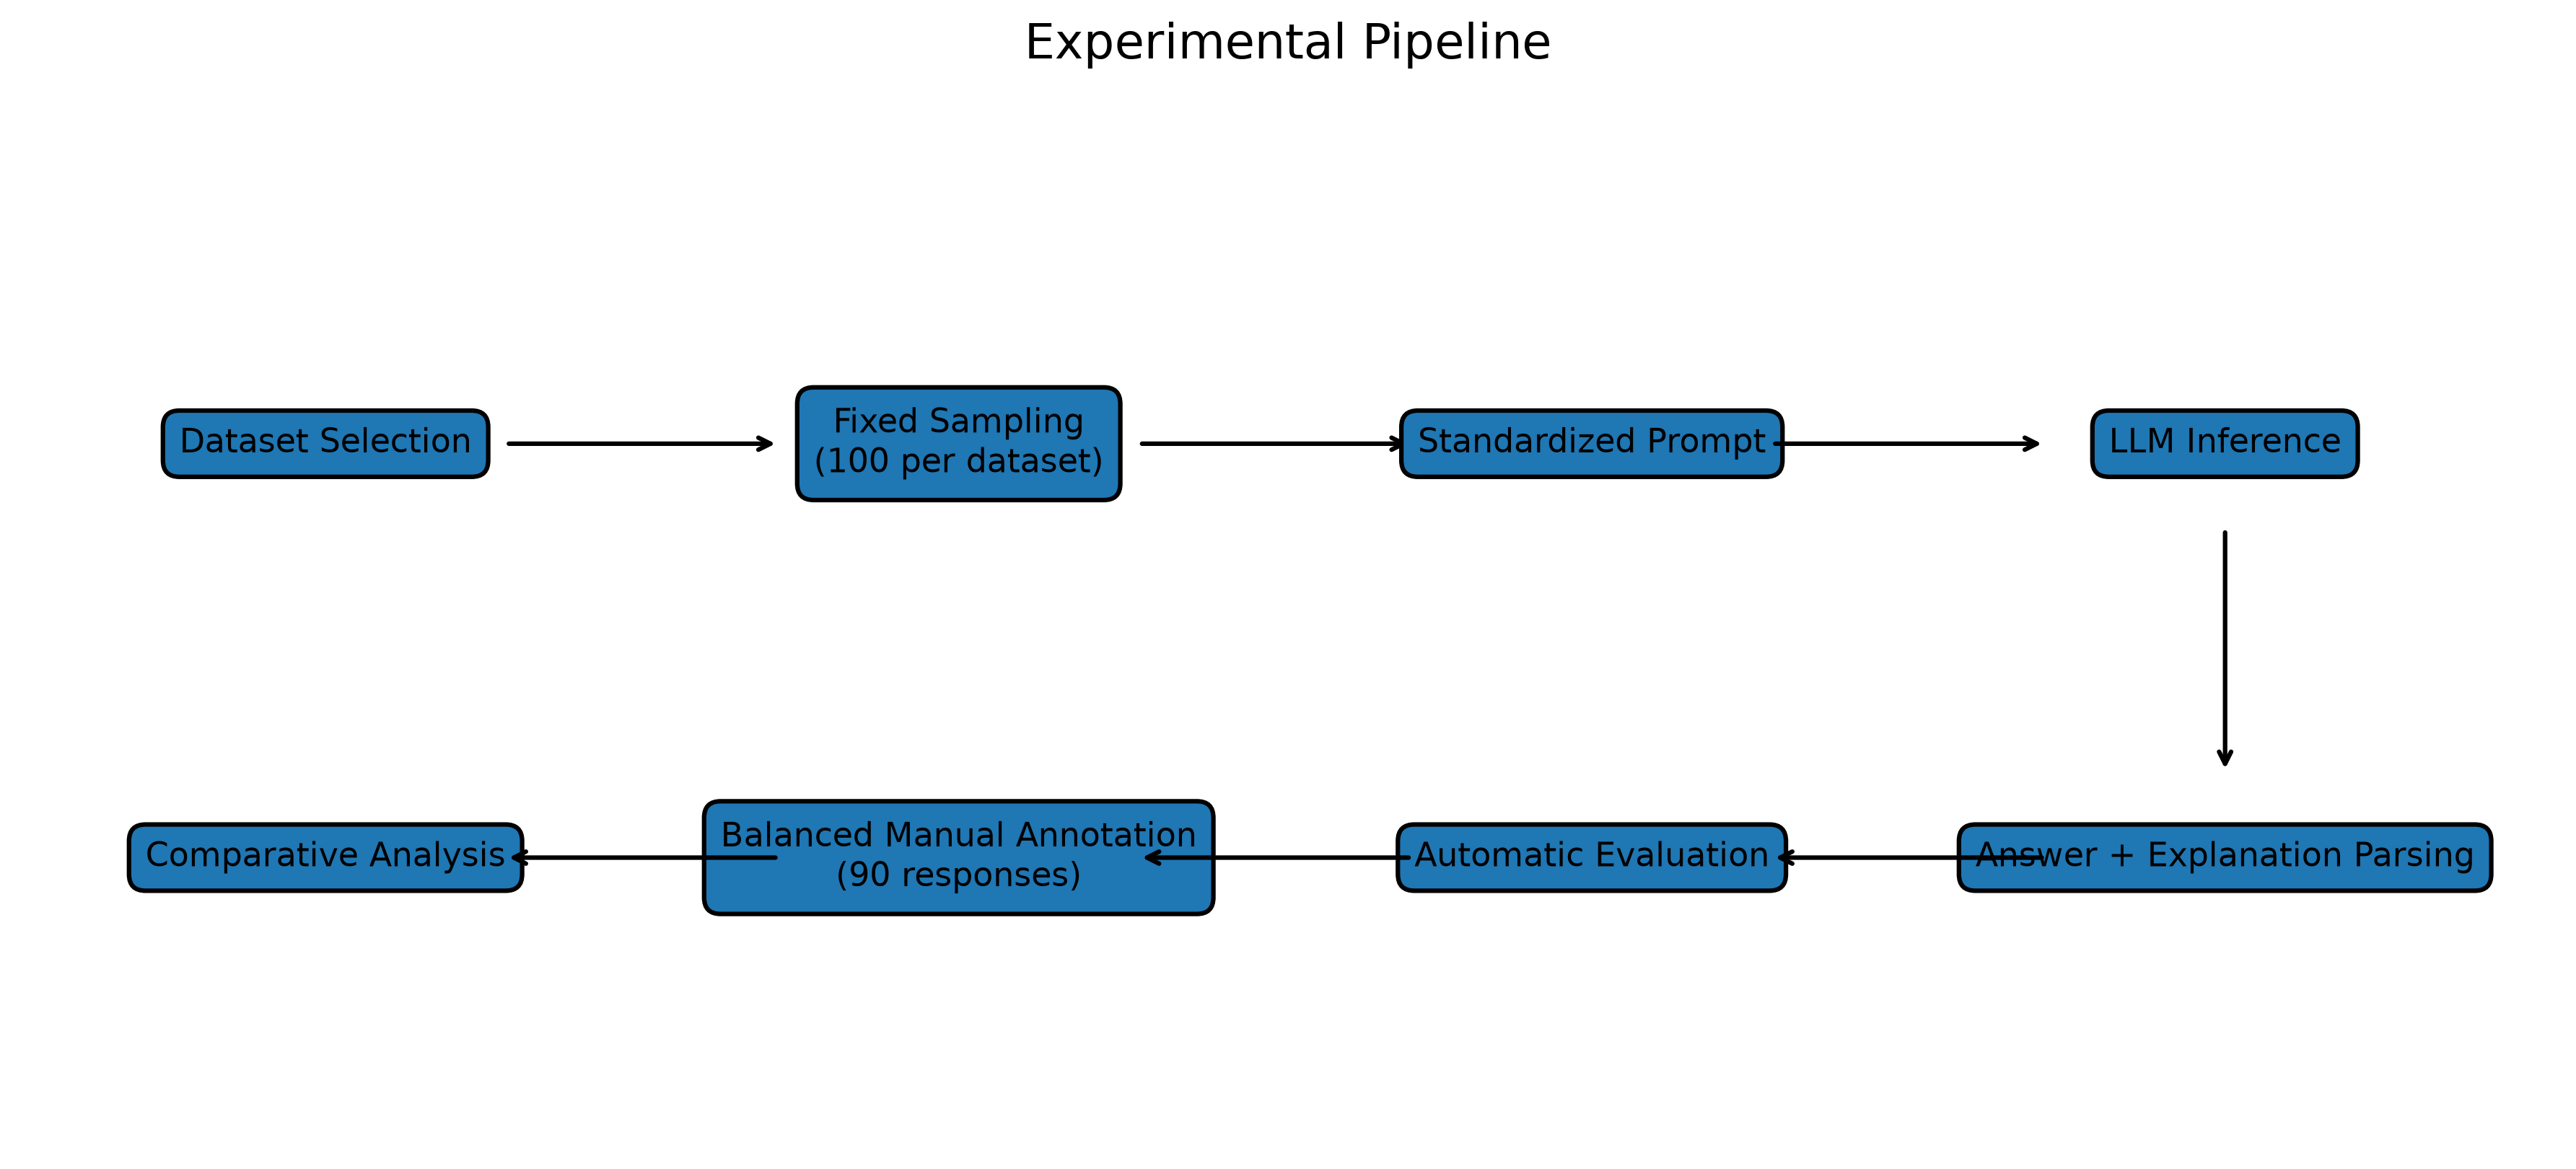
\includegraphics[width=\textwidth]{experimental_pipeline.png}
    \caption{Experimental pipeline. Each model was evaluated on 100 fixed samples from each dataset, followed by automatic answer evaluation and balanced manual annotation of 90 explanations.}
    \label{fig:pipeline}
\end{figure}

The design separates four evaluation dimensions: predictive performance, instruction compliance, computational efficiency, and explanation quality. This separation is important because a model can be accurate but difficult to parse, fast but incomplete, or internally coherent while supporting an incorrect final answer.

\subsection{Research Questions and Operationalization}

RQ1 is operationalized through answer accuracy for each model--dataset pair and overall. RQ2 is evaluated using strict parse success, defined as the presence of both required fields in the prescribed structure. RQ3 is evaluated using manual 0--3 scores for explanation-support faithfulness, logical consistency, and completeness. RQ4 is examined through a primary failure taxonomy applied to the manually annotated subset.

\subsection{Selected Open-Source Models}

Table~\ref{tab:models} lists the evaluated models. The selection includes two general instruction-tuned models of approximately 3B parameters and one smaller reasoning-distilled model. This design permits comparison between broadly capable instruction models and a model optimized for explicit reasoning.

\begin{table}[h]
\centering
\caption{Evaluated open-source language models.}
\label{tab:models}
\begin{tabular}{lll}
\toprule
\textbf{Model} & \textbf{Model identifier} & \textbf{Quantization} \\
\midrule
Qwen 2.5 3B &
\texttt{Qwen/Qwen2.5-3B-Instruct} &
4-bit NF4 \\
Llama 3.2 3B &
\texttt{meta-llama/Llama-3.2-3B-Instruct} &
4-bit NF4 \\
DeepSeek-R1 Distill 1.5B &
\texttt{deepseek-ai/DeepSeek-R1-Distill-Qwen-1.5B} &
4-bit NF4 \\
\bottomrule
\end{tabular}
\end{table}

Qwen~2.5 is a multilingual instruction-tuned family designed for broad language and reasoning tasks \cite{qwen2024qwen25}. Llama~3.2~3B is a compact instruction model derived from the Llama~3 family \cite{grattafiori2024llama3}. DeepSeek-R1 Distill Qwen~1.5B is a reasoning-oriented distilled model derived from DeepSeek-R1 \cite{deepseek2025r1}. All models were loaded with 4-bit NF4 quantization because the experiments were executed on a 4\,GB consumer GPU.

\subsection{Reasoning Datasets}

The benchmark contains three datasets representing complementary reasoning demands:

\begin{itemize}
    \item \textbf{GSM8K} contains grade-school mathematical word problems requiring arithmetic and multi-step numerical reasoning \cite{cobbe2021gsm8k}.
    \item \textbf{CommonsenseQA} contains five-option multiple-choice questions that require ordinary world knowledge and semantic associations \cite{talmor2019commonsenseqa}.
    \item \textbf{StrategyQA} contains yes/no questions whose answers often require implicit decomposition and multiple supporting facts \cite{geva2021strategyqa}.
\end{itemize}

Exactly 100 examples were sampled from each dataset. GSM8K used the test split, CommonsenseQA used the validation split, and StrategyQA used the available training split from a Parquet-compatible distribution. The final CSV and JSONL benchmark files were checksummed before final inference to support reproducibility.

\subsection{Prompt Design}

Every model received the same standardized instruction:

\begin{quote}
\texttt{FINAL\_ANSWER: <answer>}\\
\texttt{EXPLANATION: <concise justification>}
\end{quote}

For GSM8K, the final answer was numerical or short text. CommonsenseQA used option labels and option text. StrategyQA used a yes/no mapping. The explanation was requested after the answer and was intentionally constrained to be concise. A common structure reduced model-specific prompt engineering and enabled deterministic parsing.

\subsection{Evaluation Protocol}

Inference was performed separately for every model--dataset pair. Outputs were written incrementally to JSONL files so interrupted runs could resume without regenerating completed samples. After generation, the parser extracted the answer and explanation fields. Scored outputs were then merged into model-level and cross-model result tables.

The evaluation protocol produced 900 responses in total:
\[
3\ \text{models} \times 3\ \text{datasets} \times 100\ \text{samples}=900.
\]

\subsection{Automatic Evaluation Metrics}

Automatic evaluation measured:

\begin{itemize}
    \item \textbf{Answer accuracy}: benchmark-specific correctness after normalization.
    \item \textbf{Strict parse success}: whether both required response fields were produced.
    \item \textbf{Generation time}: elapsed inference time per response.
    \item \textbf{Explanation length}: number of words in the extracted explanation.
\end{itemize}

GSM8K answers were normalized numerically. CommonsenseQA answers were evaluated by option label. StrategyQA answers were mapped between \texttt{A/B}, \texttt{yes/no}, and \texttt{true/false}. Strict parse success was retained as a separate metric rather than silently recovering every malformed output, because format compliance is part of practical instruction following.

\subsection{Manual Explanation Analysis}

A balanced subset of 90 parseable responses was selected for manual analysis. The sample contained 10 responses for every model--dataset pair, with five correct and five incorrect answers whenever possible. Each model therefore contributed 30 annotated responses.

Each explanation was scored from 0 to 3 on three dimensions:

\begin{table}[h]
\centering
\caption{Manual explanation-scoring rubric.}
\label{tab:rubric}
\begin{tabular}{cl}
\toprule
\textbf{Score} & \textbf{Interpretation} \\
\midrule
0 & Contradictory, unrelated, or no meaningful reasoning \\
1 & Major errors or very weak support \\
2 & Partial support with missing or flawed reasoning \\
3 & Clear, correct, and sufficient support \\
\bottomrule
\end{tabular}
\end{table}

The same ordinal scale was applied to explanation-support faithfulness, logical consistency, and completeness. A primary failure label was additionally assigned from: answer--explanation mismatch, arithmetic error, contradictory explanation, factual hallucination, incomplete reasoning, instruction-following failure, logical error, unsupported justification, other, or no primary failure.

The annotation measures visible behavioral support. It does not establish that the textual explanation is causally identical to the hidden computation used by the model. This distinction follows prior warnings about over-interpreting generated rationales \cite{turpin2023language,lanham2023measuring}.

\section{Experimental Setup}

The experimental setup was designed to maximize reproducibility within the constraints of local consumer hardware. Model configuration, benchmark sampling, prompts, generated outputs, and scoring files were stored in a version-controlled project structure.

\subsection{Hardware and Software}

Experiments were conducted on Windows using Python~3.11.2, PyTorch~2.7.1 with CUDA~11.8, and an NVIDIA GeForce GTX~1650~Ti with 4\,GB VRAM. Hugging Face Transformers, Datasets, bitsandbytes, Accelerate, Pandas, and Matplotlib were used for inference, preprocessing, scoring, and visualization.

\subsection{Model Configuration}

All models used their official Hugging Face chat templates and automatic device placement. The tokenizer padding token was mapped to the end-of-sequence token when required. Quantized loading used bitsandbytes NF4 with double quantization and float16 computation.

\subsection{Generation Settings}

Greedy deterministic decoding was used for reproducibility. Sampling was disabled and the random seed was fixed to 42. Qwen and Llama used a maximum of 256 new tokens. DeepSeek initially failed to complete many responses under this limit because of long reasoning traces; its final run therefore used 768 new tokens. This difference is reported explicitly because it affects runtime and format compliance.

\begin{table}[h]
\centering
\caption{Generation configuration.}
\label{tab:generation}
\begin{tabular}{ll}
\toprule
\textbf{Parameter} & \textbf{Value} \\
\midrule
Decoding & Greedy \\
Sampling & Disabled \\
Temperature & 0.0 \\
Random seed & 42 \\
Qwen/Llama maximum new tokens & 256 \\
DeepSeek maximum new tokens & 768 \\
Quantization & 4-bit NF4 \\
\bottomrule
\end{tabular}
\end{table}



\subsection{Experimental Procedure}

For each model, one pilot example was first generated to confirm loading, formatting, and parsing. The final run then generated 100 responses per dataset. Greedy decoding ensured that rerunning a completed sample under the same settings produced the same response. Model outputs were scored separately for each dataset and then combined into a 900-row master results file.

DeepSeek initially used the same 256-token limit as the other models, but many responses were truncated before reaching the required output fields. Inspection of raw outputs showed that the model was still producing long reasoning traces when generation stopped. The final DeepSeek run therefore used 768 new tokens. The larger budget improved parse success but increased inference time.

\subsection{Reproducibility}

The final benchmark was generated with seed 42 and stored in both CSV and JSONL formats. A SHA-256 checksum was recorded after StrategyQA was added. Output files preserve the sample identifier, model identifier, prompt, raw generation, parsed answer, explanation, timing, parse status, and error field. The code and experiment artifacts are maintained in the FaithfulLLM repository.

\section{Results}

\subsection{Answer Accuracy}

Table~\ref{tab:accuracy} and Figure~\ref{fig:accuracy} show answer accuracy for all model--dataset combinations.

\begin{table}[h]
\centering
\caption{Answer accuracy (\%) by model and dataset.}
\label{tab:accuracy}
\begin{tabular}{lrrrr}
\toprule
\textbf{Model} & \textbf{GSM8K} & \textbf{CSQA} & \textbf{StrategyQA} & \textbf{Overall} \\
\midrule
Qwen 2.5 3B & 13 & 76 & 60 & 49.67 \\
Llama 3.2 3B & 6 & 70 & 59 & 45.00 \\
DeepSeek-R1 Distill 1.5B & 80 & 28 & 49 & 52.33 \\
\bottomrule
\end{tabular}
\end{table}

\begin{figure}[t]
    \centering
    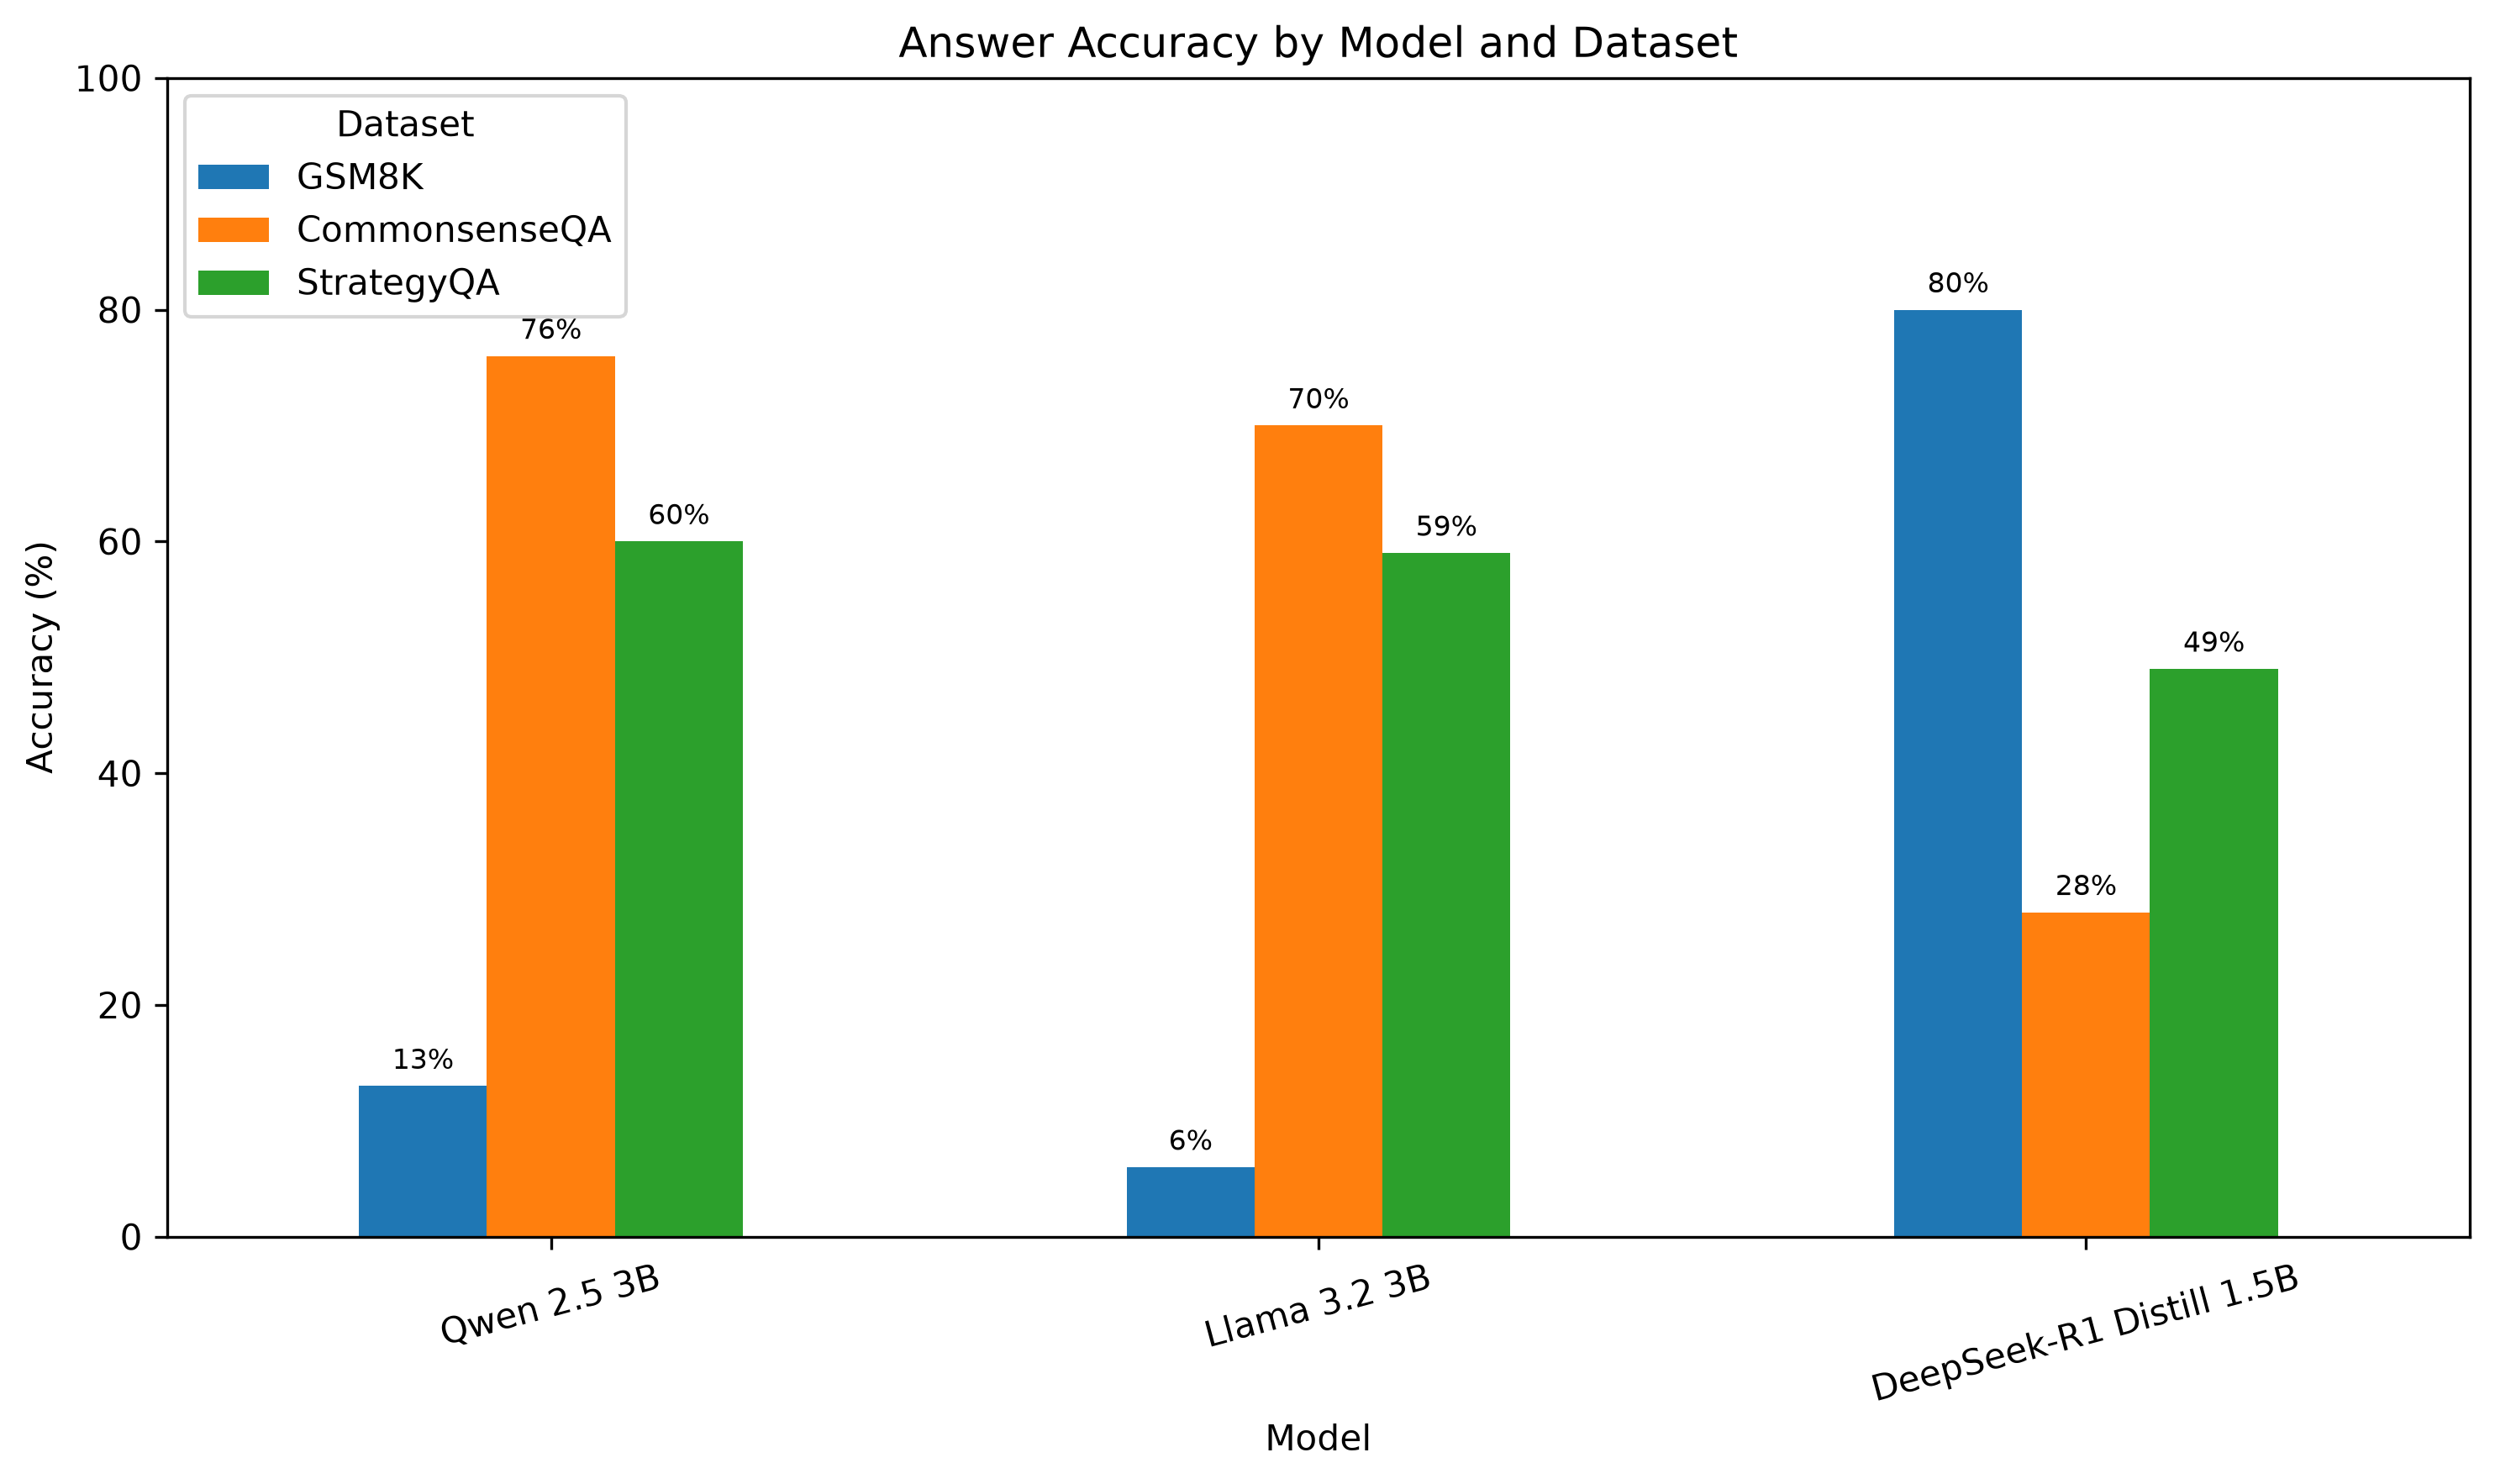
\includegraphics[width=\textwidth]{accuracy_by_model_dataset.png}
    \caption{Answer accuracy by model and dataset. DeepSeek-R1 Distill performs best on GSM8K, whereas Qwen~2.5 performs best on CommonsenseQA and StrategyQA.}
    \label{fig:accuracy}
\end{figure}

The results reveal strong task specialization. DeepSeek-R1 Distill achieved 80\% on GSM8K, far above Qwen (13\%) and Llama (6\%). In contrast, Qwen achieved the best CommonsenseQA accuracy (76\%) and the best StrategyQA accuracy (60\%). Llama followed closely on CommonsenseQA (70\%) and StrategyQA (59\%) but performed poorly on GSM8K.

\subsection{Format Compliance and Runtime}

Table~\ref{tab:efficiency} reports strict parse success and mean generation time. Llama followed the required format for all responses. Qwen failed on only two CommonsenseQA outputs. DeepSeek achieved the lowest strict parse success because several responses contained long reasoning loops, incomplete outputs, or a final answer without the required explanation field.

\begin{table}[h]
\centering
\caption{Overall strict parse success and mean generation time.}
\label{tab:efficiency}
\begin{tabular}{lrr}
\toprule
\textbf{Model} & \textbf{Parse success (\%)} & \textbf{Mean time (s)} \\
\midrule
Qwen 2.5 3B & 99.33 & 10.21 \\
Llama 3.2 3B & 100.00 & 7.57 \\
DeepSeek-R1 Distill 1.5B & 85.67 & 37.01 \\
\bottomrule
\end{tabular}
\end{table}

DeepSeek was substantially slower because of its longer reasoning traces and higher token limit. Its strong mathematical performance therefore came with a clear efficiency and instruction-compliance cost.

\subsection{Manual Explanation Scores}

Table~\ref{tab:manual_scores} summarizes mean manual scores across 30 annotated responses per model.

\begin{table}[h]
\centering
\caption{Mean manual explanation scores on a 0--3 scale.}
\label{tab:manual_scores}
\begin{tabular}{lrrr}
\toprule
\textbf{Model} & \textbf{Faithfulness} & \textbf{Logic} & \textbf{Completeness} \\
\midrule
DeepSeek-R1 Distill 1.5B & 1.87 & 2.07 & 2.03 \\
Llama 3.2 3B & 1.70 & 2.20 & 2.17 \\
Qwen 2.5 3B & 1.73 & 2.13 & 2.30 \\
\bottomrule
\end{tabular}
\end{table}

DeepSeek obtained the highest average explanation-support faithfulness score. Llama achieved the highest logical-consistency score, while Qwen produced the most complete explanations. The differences are moderate and do not support a claim that one model is uniformly best.

\subsection{Faithfulness by Dataset}

Figure~\ref{fig:faithfulness_heatmap} shows substantial task-dependent variation. DeepSeek achieved the highest faithfulness on CommonsenseQA (2.40) and GSM8K (2.10), but the lowest score on StrategyQA (1.10). Llama and Qwen both achieved 1.70 on StrategyQA, while their GSM8K explanations scored 1.40 and 1.30 respectively.

\begin{figure}[t]
    \centering
    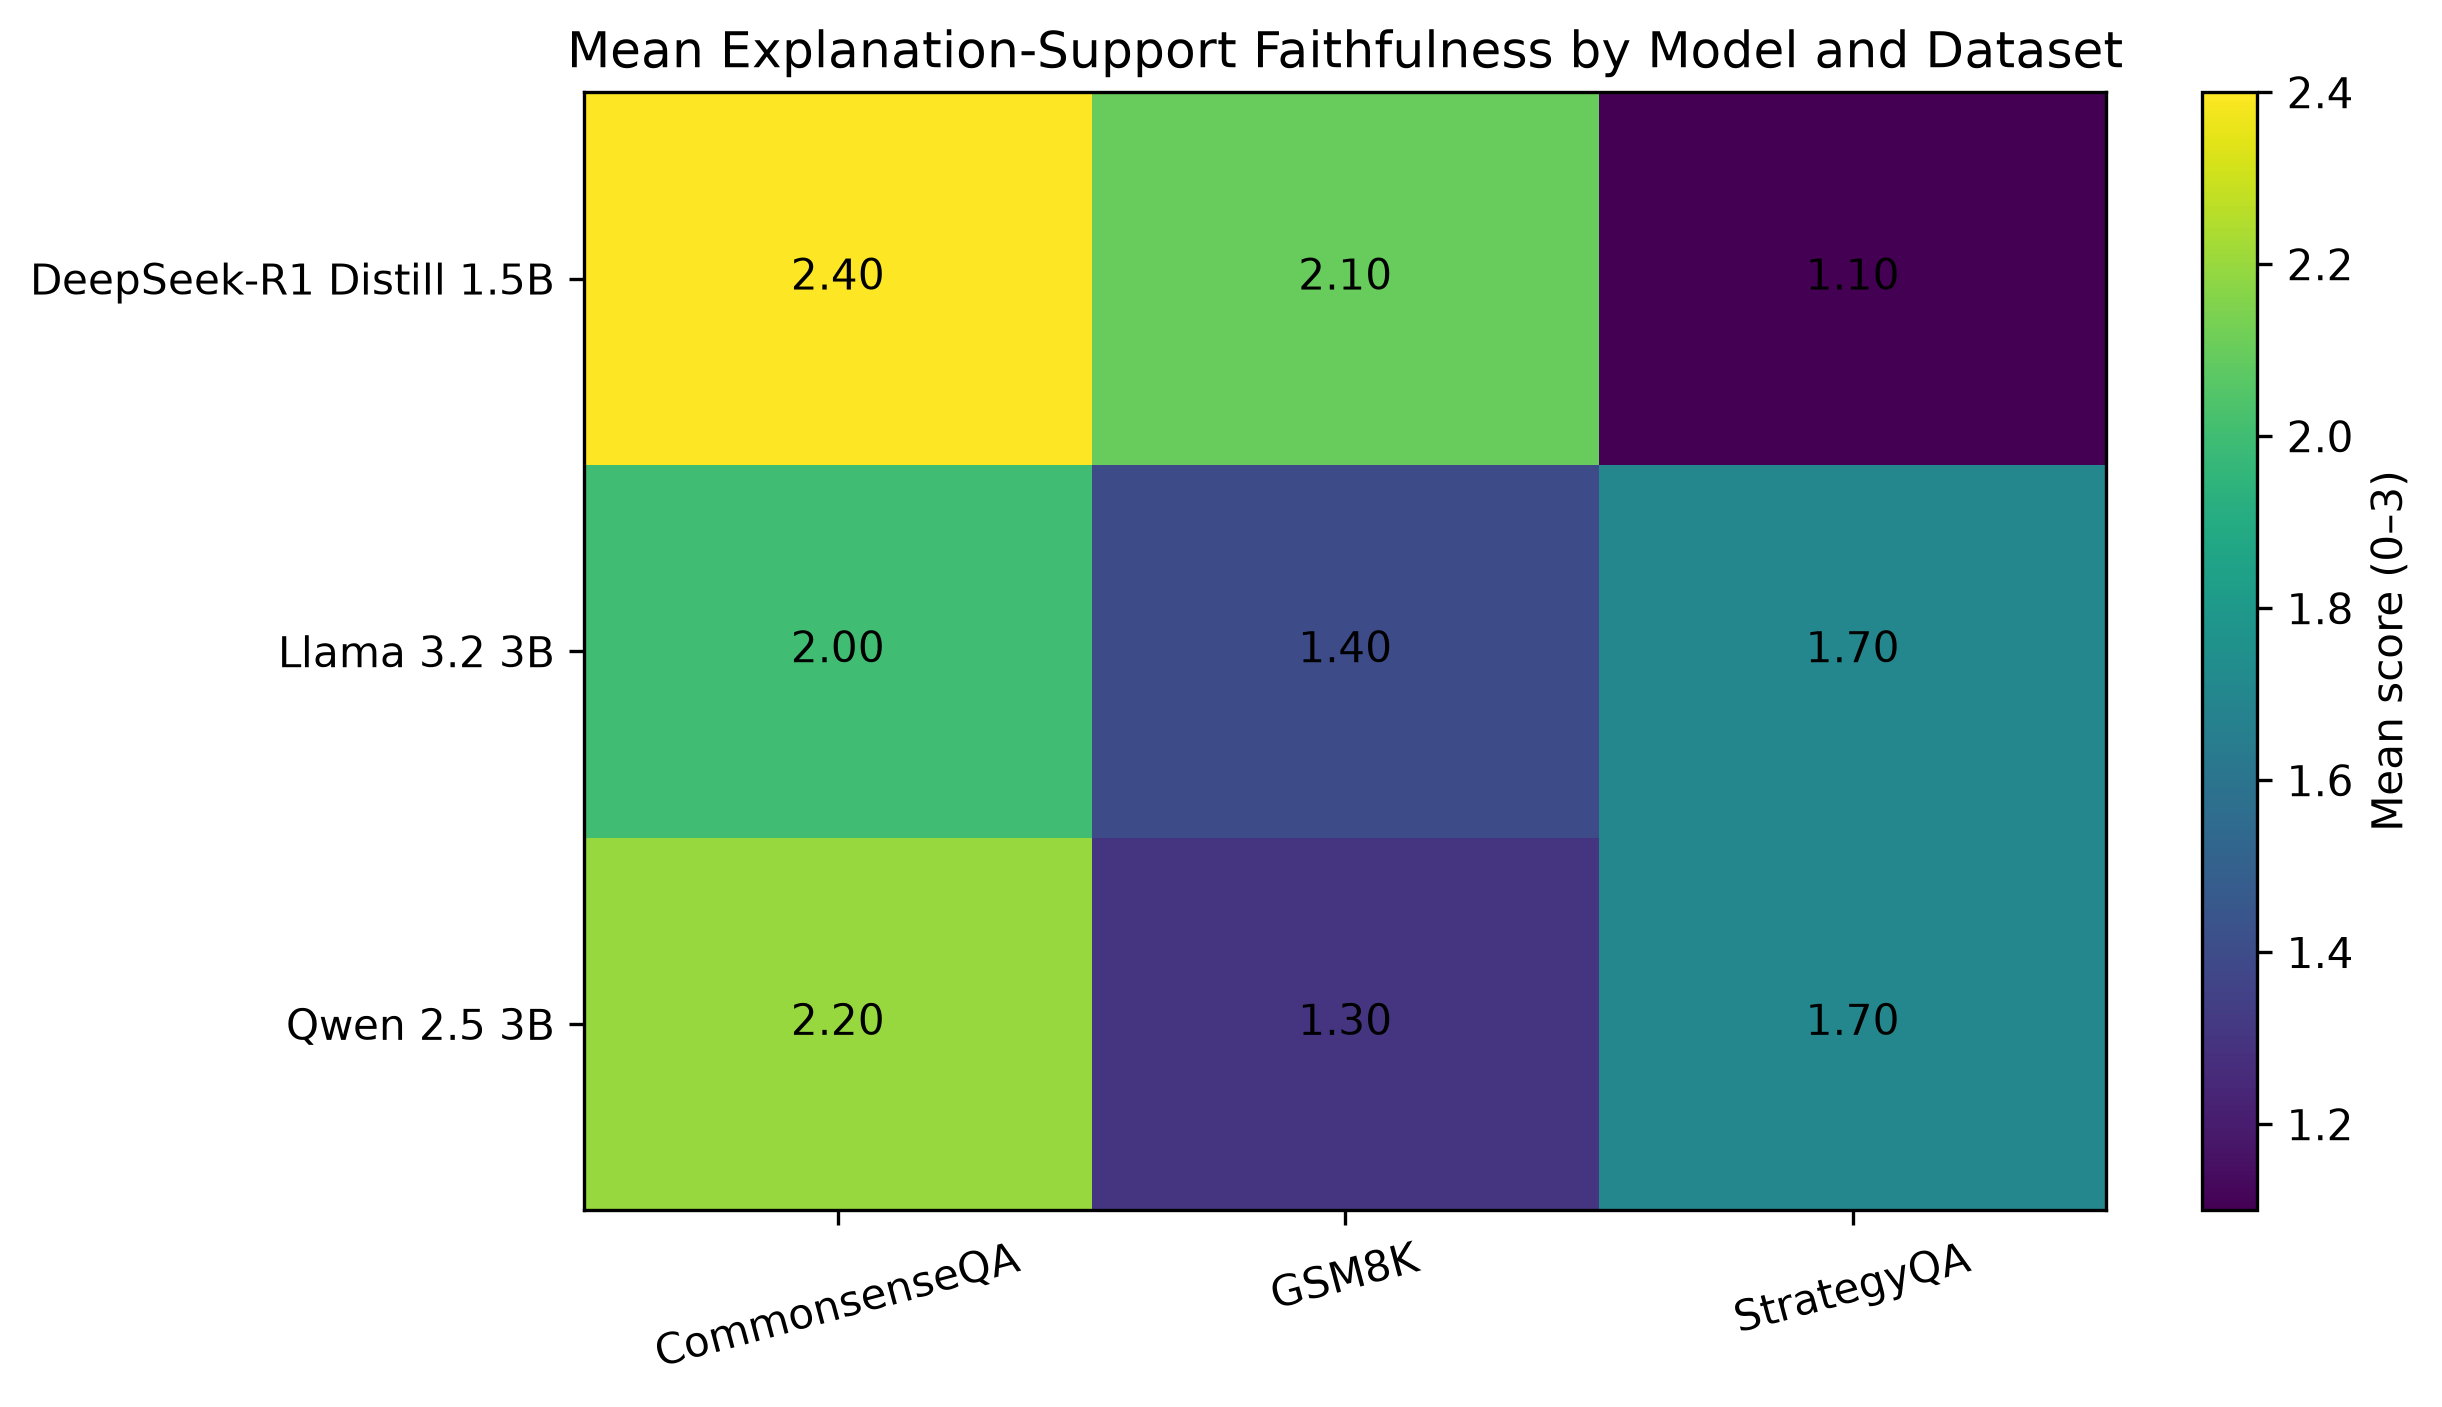
\includegraphics[width=\textwidth]{faithfulness_heatmap.png}
    \caption{Mean explanation-support faithfulness score by model and dataset. The values show strong task-dependent differences in explanation quality.}
    \label{fig:faithfulness_heatmap}
\end{figure}

\subsection{Correct vs.\ Incorrect Answers}

Figure~\ref{fig:correct_incorrect} presents one of the clearest findings. Explanations accompanying correct answers received much higher faithfulness scores than explanations accompanying incorrect answers for every model.

\begin{figure}[t]
    \centering
    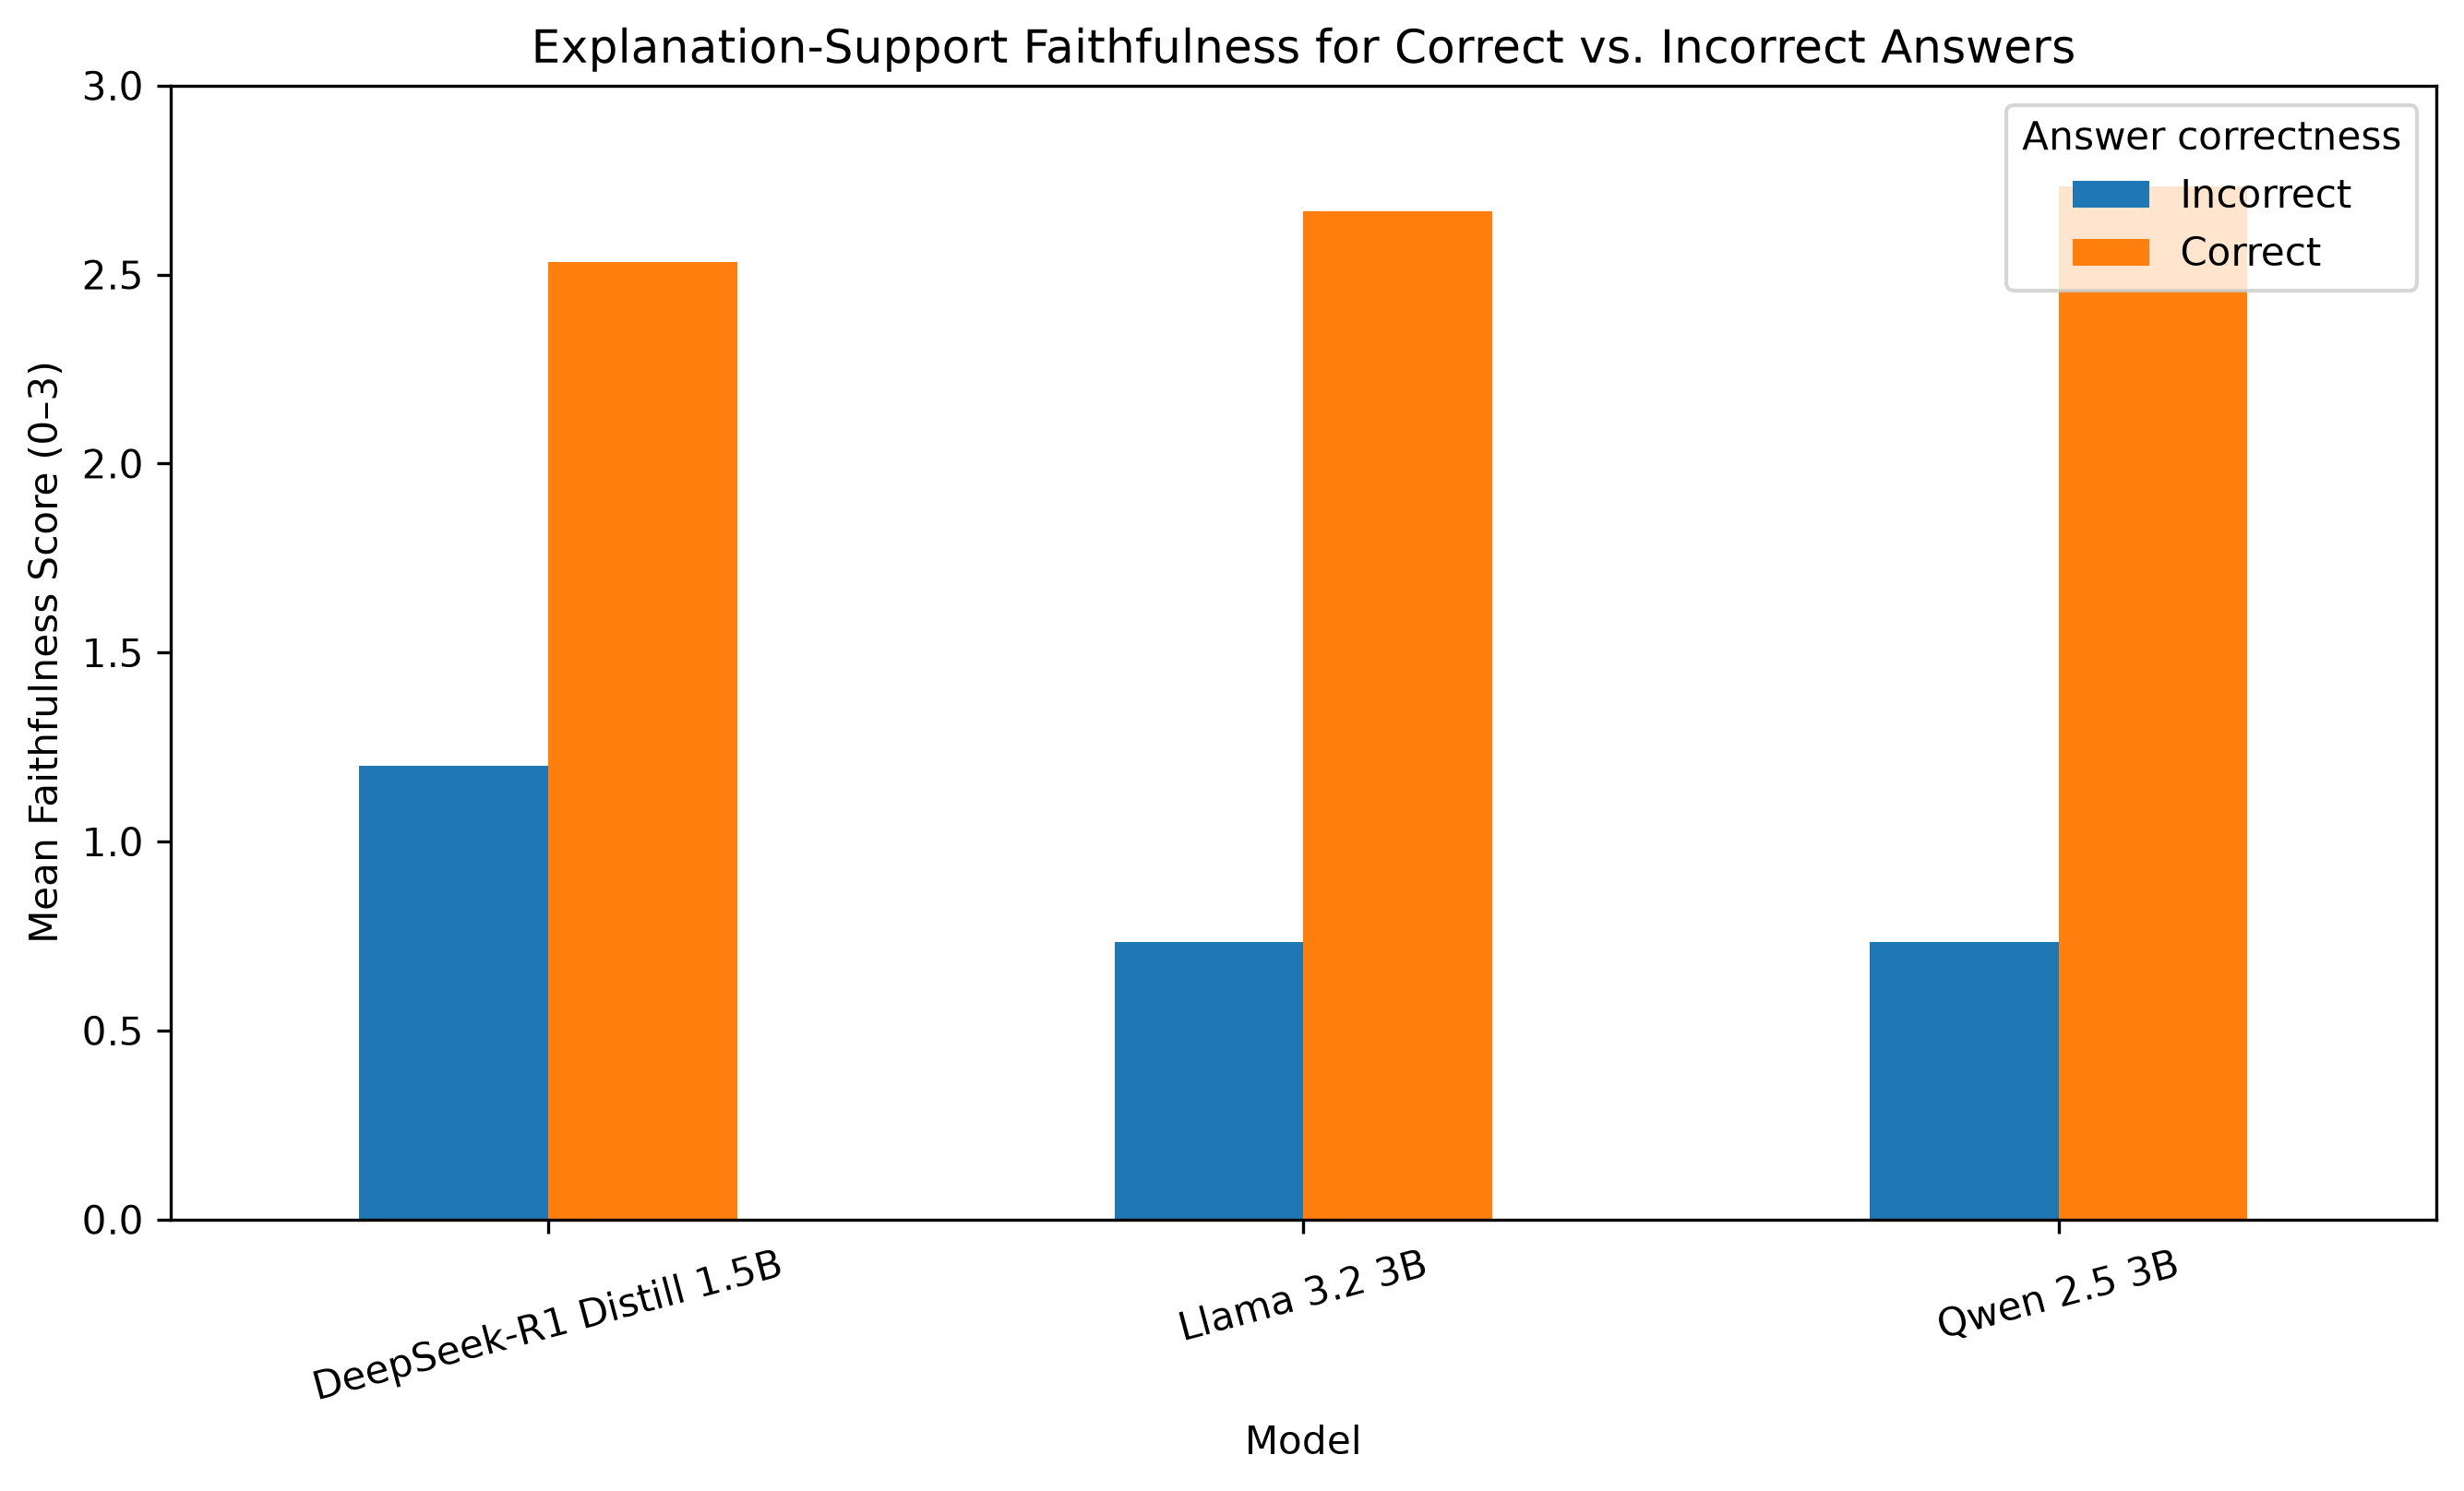
\includegraphics[width=\textwidth]{faithfulness_correct_vs_incorrect.png}
    \caption{Mean explanation-support faithfulness for correct and incorrect answers. Correct answers receive substantially higher scores across all evaluated models.}
    \label{fig:correct_incorrect}
\end{figure}

For DeepSeek, the mean score increased from 1.20 for incorrect answers to 2.53 for correct answers. Llama increased from 0.73 to 2.67, and Qwen from 0.73 to 2.73. Correctness is therefore strongly associated with better visible explanations, although a correct answer alone does not prove faithful internal reasoning.

\subsection{Failure Categories}

Figure~\ref{fig:failure_categories} summarizes the primary failure types in the balanced manual sample.

\begin{figure}[t]
    \centering
    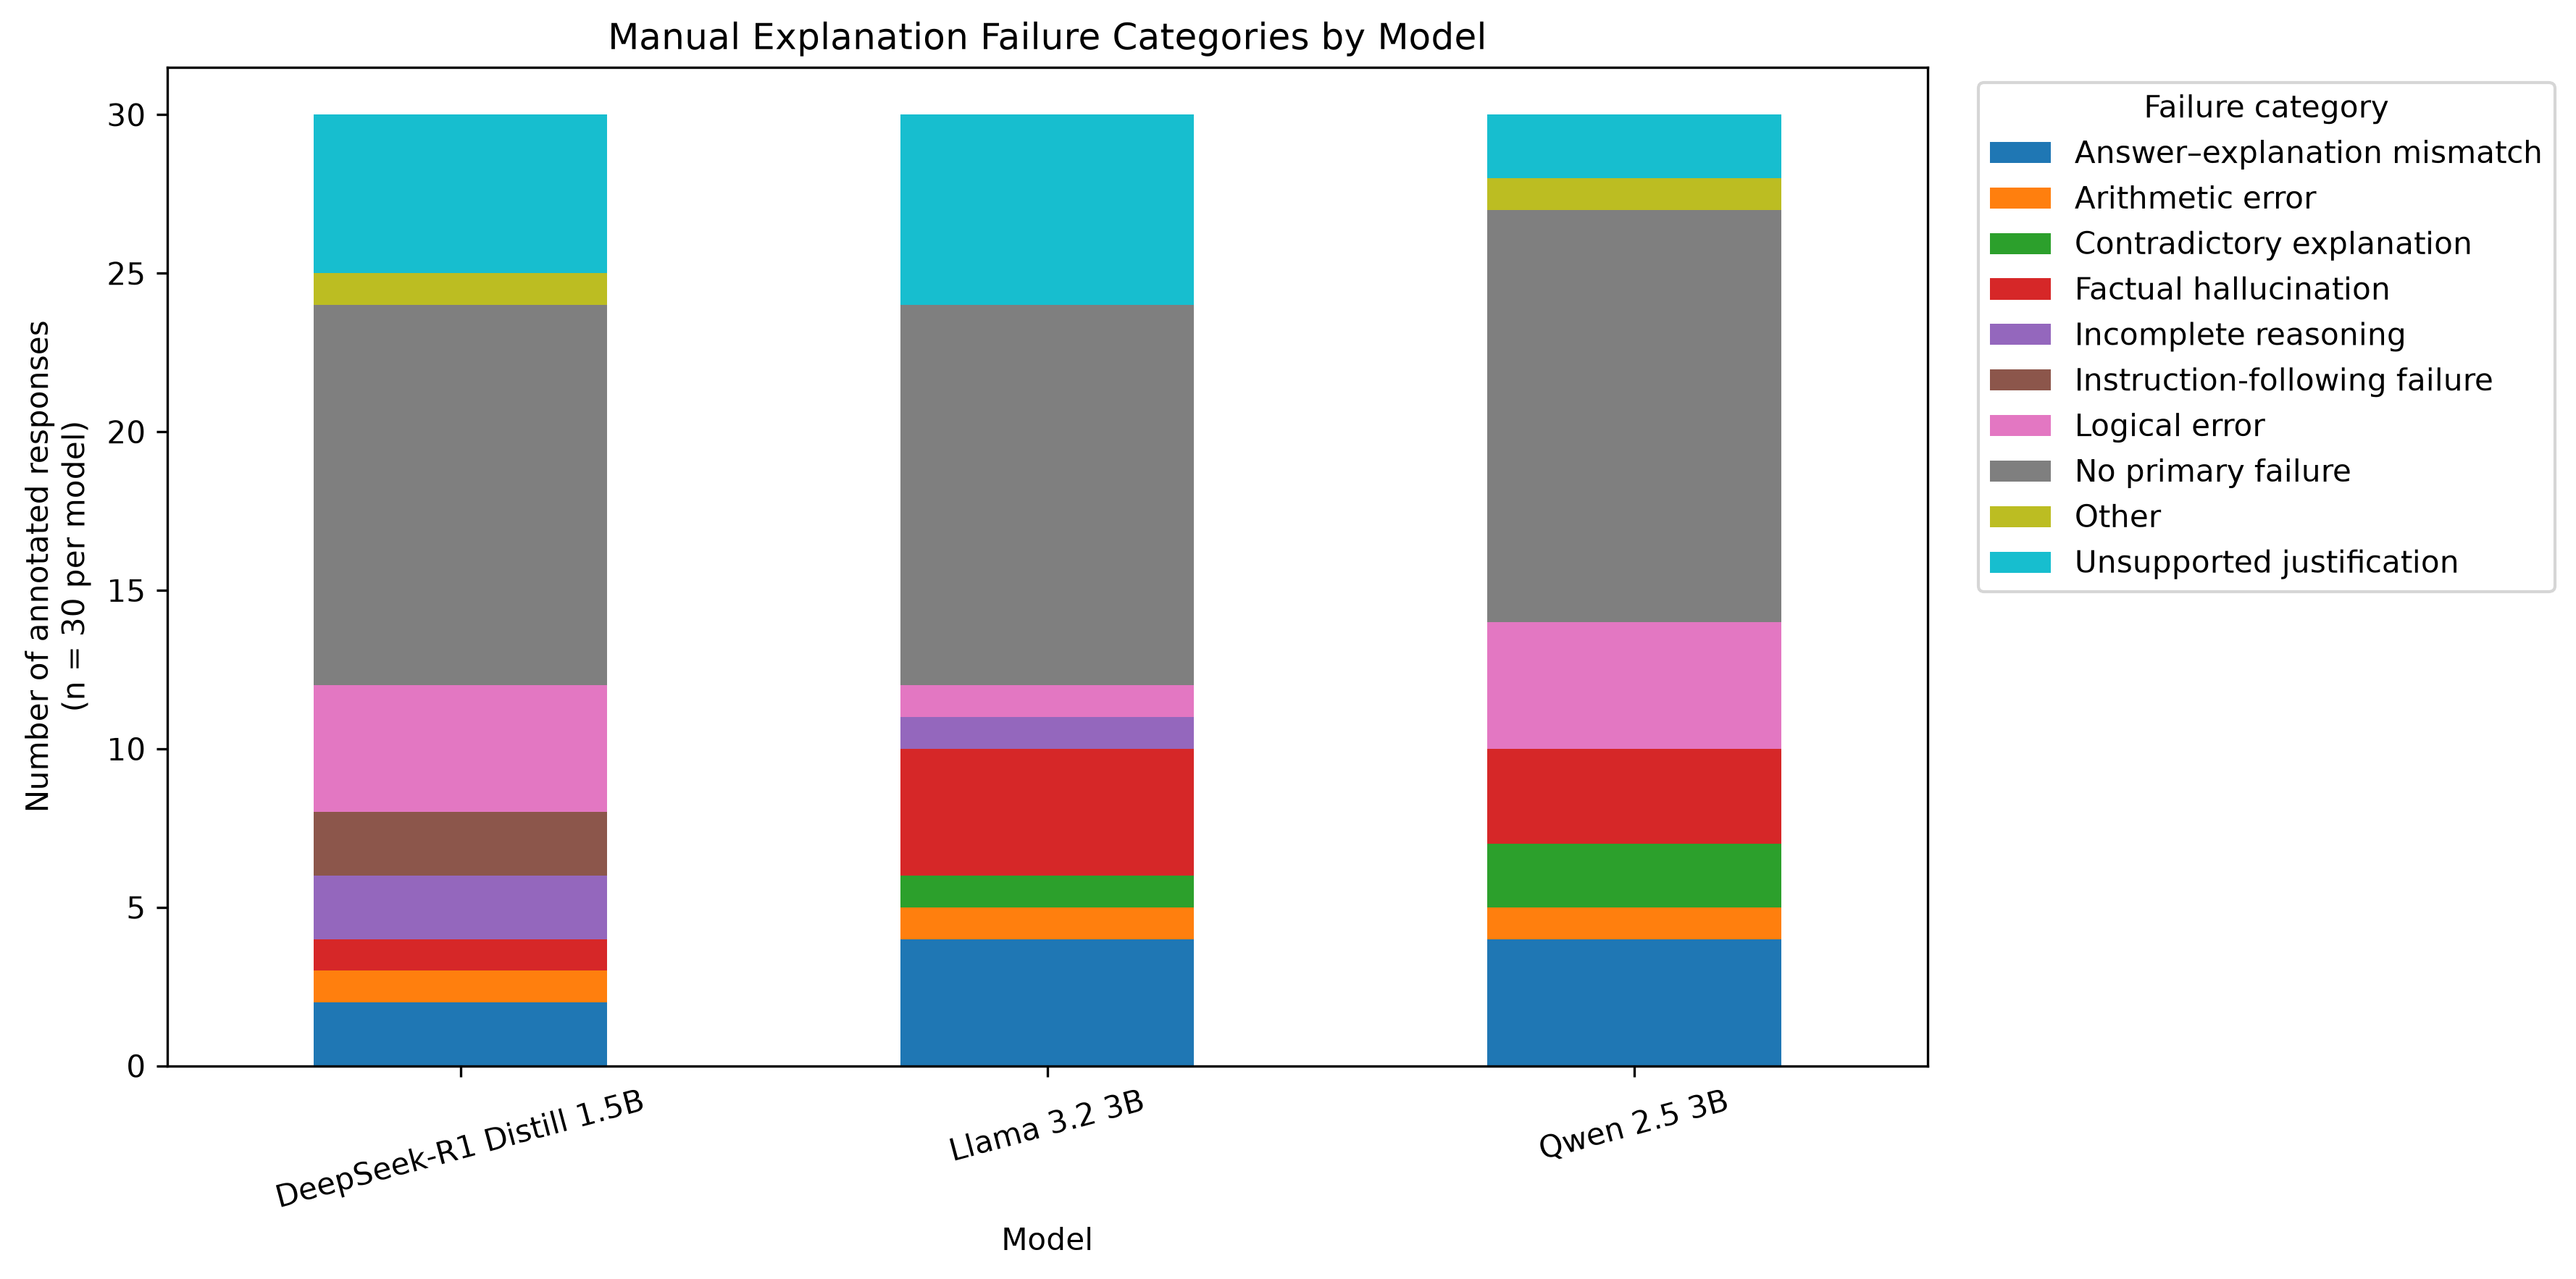
\includegraphics[width=\textwidth]{failure_categories_by_model.png}
    \caption{Primary explanation failure categories in the balanced manual annotation sample ($n=30$ per model).}
    \label{fig:failure_categories}
\end{figure}

Unsupported justification was common for DeepSeek and Llama. Llama and Qwen exhibited several factual hallucinations and answer--explanation mismatches. Qwen additionally showed contradictory explanations, particularly on GSM8K, where the explanation sometimes reached the correct numerical result while the final answer contained a different value.

A representative mismatch occurred when a model explanation correctly computed a total duration of 70 minutes but returned 220 as its final answer. Another response correctly derived a value of 13 in the explanation but returned 10. Such cases are especially important because the explanation appears competent while the final prediction is inconsistent with it.




\subsection{Statistical Analysis}

Wilson confidence intervals were calculated for answer accuracy.
Because the manual faithfulness ratings were ordinal scores on a
0--3 scale, correct and incorrect answers were compared using a
two-sided Mann--Whitney U test. Cliff's delta was used to quantify
effect size, and a non-parametric bootstrap with 10,000 resamples
was used to estimate a 95\% confidence interval for the difference
in mean faithfulness scores.

Across all models, explanations accompanying correct answers obtained
a mean explanation-support faithfulness score of 2.64, compared with
0.89 for explanations accompanying incorrect answers. The mean
difference was 1.76 points, with a bootstrap 95\% confidence interval
of [1.42, 2.07]. The score distributions differed significantly
($U=1827.0$, $p<0.001$), and Cliff's delta was 0.804, indicating a
large effect.

The effect remained large for each model individually. Qwen achieved
a mean difference of 2.00 points
($U=214.0$, $p<0.001$, $\delta=0.902$), while Llama achieved a
difference of 1.93 points
($U=211.5$, $p<0.001$, $\delta=0.880$). DeepSeek showed a smaller but
still large difference of 1.33 points
($U=183.0$, $p=0.001$, $\delta=0.627$).

These results show a strong association between answer correctness
and visible explanation quality. However, they do not demonstrate
that the explanations causally reflect the models' internal reasoning
processes.

At the overall level, DeepSeek-R1 Distill obtained the highest observed
accuracy at 52.33\% (95\% CI: 46.69--57.92), followed by Qwen 2.5 at
49.67\% (95\% CI: 44.05--55.29) and Llama 3.2 at 45.00\%
(95\% CI: 39.47--50.66). Because these intervals overlap substantially,
the observed overall differences should not be interpreted as decisive
evidence that one model is universally superior.

The dataset-level results reveal clearer specialization. DeepSeek
achieved 80.00\% on GSM8K (95\% CI: 71.12--86.66), whereas Qwen and
Llama achieved 13.00\% and 6.00\%, respectively. In contrast, Qwen
performed best on CommonsenseQA with 76.00\%
(95\% CI: 66.77--83.31) and slightly outperformed Llama and DeepSeek
on StrategyQA with 60.00\% accuracy.

\subsection{Results Summary}

The quantitative and manual results jointly support the three hypotheses. First, performance is strongly task-specific rather than uniform: DeepSeek is dominant on GSM8K, while Qwen and Llama are stronger on CommonsenseQA and StrategyQA. Second, correct answers receive substantially higher explanation-support faithfulness scores than incorrect answers for every model. Third, DeepSeek's reasoning specialization brings a practical trade-off: its mathematical accuracy is high, but it is slower and less reliable in strict output formatting.

No single metric is sufficient to rank the models. Overall answer accuracy favors DeepSeek, format compliance favors Llama, balanced task performance favors Qwen, and the manual analysis reveals different strengths in faithfulness, consistency, and completeness.

\section{Discussion}

\subsection{Task Specialization}

The results show that no model is consistently best across tasks. DeepSeek-R1 Distill is strongly specialized for mathematical reasoning, while Qwen and Llama are stronger on commonsense and strategy questions. This specialization also appears in explanation quality. DeepSeek's GSM8K explanations are comparatively strong, but its StrategyQA explanations are weak and often rely on unsupported or hallucinated claims.

\subsection{Accuracy and Explanation Quality}

Answer accuracy and explanation quality are related but distinct. Correct answers usually receive high explanation-support scores, yet the models still produce correct answers with weak reasoning and incorrect answers with fluent explanations. The balanced analysis makes this difference visible because it prevents the manual sample from being dominated by easy correct cases.

The observed answer--explanation mismatches are particularly concerning. A user may read a correct-looking chain of reasoning and overlook that the stated final answer is inconsistent. Conversely, a model can provide a confident but unsupported explanation for an incorrect answer. Therefore, explanation fluency should not be treated as a substitute for answer verification.

\subsection{Instruction Compliance}

Strict format success was nearly perfect for Qwen and Llama but lower for DeepSeek. DeepSeek frequently generated long internal-style reasoning traces, repeated itself, or failed to reach the required output fields within the token budget. Increasing the token limit improved completion rates but increased runtime substantially. This trade-off matters for practical deployment: a reasoning-oriented model may solve difficult tasks well while remaining less predictable and more expensive to evaluate.

\subsection{Comparison with Previous Work}

The observed gap between fluent explanation and reliable support is consistent with prior work showing that chain-of-thought text can be influenced by irrelevant prompt features and can function as a post-hoc rationale \cite{turpin2023language,lanham2023measuring}. The strong correct-versus-incorrect difference also aligns with studies that treat explanation quality as related to, but not identical with, prediction quality \cite{madsen2024selfexplanations,paul2024making}.

The results additionally complement broad benchmarking work by showing why aggregate accuracy alone is insufficient \cite{liang2023helm}. DeepSeek's overall accuracy is highest, yet its strict parse success and runtime are substantially worse. Conversely, Llama's perfect format compliance does not translate into strong mathematical accuracy. This demonstrates that trustworthy model selection requires multiple criteria rather than a single leaderboard score.

\subsection{Implications for XAI}

The findings support a cautious interpretation of LLM self-explanations. The manual scores capture whether an explanation supports the visible answer, not whether it exposes the hidden causal computation of the neural network. Consequently, these explanations are best viewed as \emph{behavioral justifications}. They can help users inspect model outputs, but they should not be presented as direct windows into internal reasoning.

For trustworthy deployment, self-explanations should be combined with independent answer verification \cite{weng2023selfverification}, uncertainty or hallucination estimation \cite{manakul2023selfcheckgpt,farquhar2024semantic}, retrieval or tool support, and consistency checks between the explanation and final answer.


\section{Limitations}

This study has several limitations.

First, only three relatively small open-source models were evaluated. The findings may not generalize to larger proprietary systems or future model families.

Second, the benchmark contains only 100 samples per dataset. Although the sample is fixed and balanced across models, a larger evaluation would reduce sampling uncertainty.

Third, manual explanation analysis was limited to 90 responses and used a single structured annotation process. The scores therefore contain subjective judgment. A stronger study would use multiple independent annotators and report inter-annotator agreement.

Fourth, the manual rubric measures explanation-support faithfulness rather than causal faithfulness. It cannot establish whether the explanation reflects the model's internal computation.

Fifth, all models were evaluated under 4-bit quantization on a 4\,GB GPU. Quantization may affect output quality, particularly for small mathematical differences. DeepSeek also required a larger generation budget than Qwen and Llama, which complicates direct efficiency comparison.

Finally, the study uses one standardized prompt. Alternative prompting strategies could change both accuracy and explanation behavior.


\section{Future Work}

Future work should extend the evaluation to larger models, additional reasoning datasets, and multilingual tasks. Multiple human annotators should be used to estimate inter-annotator agreement. Stronger causal tests could perturb problem values, reorder options, remove rationale steps, or intervene on generated explanations to test whether answers change appropriately \cite{lanham2023measuring,matton2025walk,zaman2025causal}. Automated detectors for answer--explanation mismatch and hallucinated justification would also improve scalable evaluation.


\section{Conclusion}

This paper evaluated self-generated explanations from Qwen~2.5~3B, Llama~3.2~3B, and DeepSeek-R1 Distill Qwen~1.5B on GSM8K, CommonsenseQA, and StrategyQA. Across 900 responses, the models showed strong task specialization: DeepSeek dominated mathematical reasoning, while Qwen performed best on commonsense and strategy tasks. Llama and Qwen followed the required output format reliably, whereas DeepSeek produced longer and less predictable outputs.

Manual analysis of 90 balanced responses showed that explanations for correct answers were substantially more faithful than explanations for incorrect answers. Nevertheless, all models produced unsupported justifications, hallucinations, arithmetic errors, contradictions, and answer--explanation mismatches. These findings demonstrate that natural-language self-explanations can be useful behavioral evidence, but they should not be interpreted as direct proof of faithful internal reasoning.

\bibliographystyle{plain}
\bibliography{references}




\appendix

\section{Standardized Prompt}
\label{app:prompt}

\section{Manual Annotation Rubric}
\label{app:rubric}

\section{Additional Statistical Results}
\label{app:statistics}

\section{Additional Qualitative Examples}
\label{app:examples}

\section{Reproducibility Details}
\label{app:reproducibility}

\end{document}
